% Fig 4 (fig:baseline_iqr): standalone source for the paper figure.
% Data provenance: three of the six series are scripted, three are not:
%   SCRIPTED (from benchmark_checkpoints/es_hyperneat_population_scaling_tables.md):
%     JAX-ESHN 30-gen band       -> extract_jaxeshn_iqr.py
%     construction overhead band -> extract_jit_iqr.py
%     construction Pop-1000 line -> extract_jit_times.py
%   NOT SCRIPTED (computed once from raw data; coordinates maintained by hand):
%     Baseline IQR band:   benchmark_checkpoints/pureples_xor_scaling/ (iteration_level==1,
%                             per-population means -> 25th/75th percentile, uniform D1-D7)
%     Baseline solve line: same source, Pop 1000: mean generations-to-solve (unsolved
%                             counted at the 30-generation cap) x mean per-generation time
%     JAX-ESHN solve line: benchmark_checkpoints/tensorneat_eshyperneat_pop1000_10gens/;
%                             D1 comes from the 300-gen campaign (unsolved at the 10-gen cap)
% CONVENTION: the JAX band is construction + 29 x per-gen, matching tab:runtime_comparison.
%   Generation 1 runs inside construction overhead (the benchmark's warm-up step), so a
%   30-generation total is construction + 29 further generations. extract_jaxeshn_iqr.py
%   already emits exactly this; paste its output unchanged.
% Build: pdflatex baseline_iqr.tex  ->  baseline_iqr.pdf  (see build_figures.sh)
% width=347.12pt matches the LLNCS \textwidth of the paper.
\documentclass[border=2pt]{standalone}
\usepackage[T1]{fontenc}
\usepackage{amsmath,amssymb}
\usepackage{tikz}
\usetikzlibrary{shapes.geometric, arrows.meta, positioning, patterns, calc}
\usepackage{pgfplots}
\pgfplotsset{compat=1.18}
\usepgfplotslibrary{fillbetween}
\usepgfplotslibrary{statistics}
% Okabe-Ito colorblind-safe palette (Wong 2011, Nature Methods)
\definecolor{oiblue}{HTML}{0072B2}
\definecolor{oiorange}{HTML}{E69F00}
\definecolor{oiskyblue}{HTML}{56B4E9}
\definecolor{oigray}{HTML}{999999}
\definecolor{oivermillion}{HTML}{D55E00}
\definecolor{oigreen}{HTML}{009E73}
\definecolor{oipurple}{HTML}{CC79A7}
\begin{document}
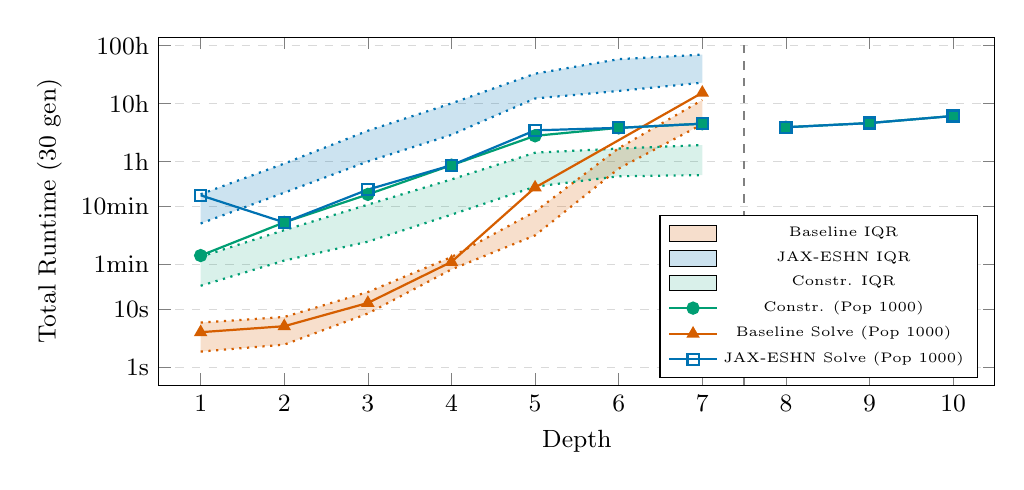
\begin{tikzpicture}
\begin{axis}[
    width=347.12pt,
    height=6cm,
    ylabel={Total Runtime (30 gen)},
    xlabel={Depth},
    ymode=log,
    ytick={1, 10, 60, 600, 3600, 36000, 360000},
    yticklabels={1s, 10s, 1min, 10min, 1h, 10h, 100h},
    ymin=0.5,
    ymax=500000,
    xmin=0.5,
    xmax=10.5,
    xtick={1,2,3,4,5,6,7,8,9,10},
    ymajorgrids=true,
    grid style={dashed, gray!30},
    tick label style={font=\small},
    label style={font=\small},
    legend style={at={(0.98,0.02)}, anchor=south east, font=\tiny},
]
% Baseline IQR band (25th-75th percentile across 8 population sizes)
\addplot[name path=baselinemin, forget plot, color=oivermillion, thick, dotted] coordinates {
    (1, 1.9) (2, 2.5) (3, 8.6) (4, 49.6) (5, 191.5) (6, 2716.6) (7, 15854.7)
};
\addplot[name path=baselinemax, forget plot, color=oivermillion, thick, dotted] coordinates {
    (1, 6.0) (2, 7.5) (3, 20.2) (4, 81.1) (5, 492.8) (6, 6100.4) (7, 41385.8)
};
\addplot[fill=oivermillion, fill opacity=0.2] fill between[of=baselinemin and baselinemax];

% JAX-ESHN IQR band (25th-75th percentile across 10 populations, 30-gen total)
\addplot[name path=jaxmin, forget plot, color=oiblue, thick, dotted] coordinates {
    (1, 307.2) (2, 1044.9) (3, 3602.9) (4, 10377.2) (5, 44035.3) (6, 59270.6) (7, 82481.7)
};
\addplot[name path=jaxmax, forget plot, color=oiblue, thick, dotted] coordinates {
    (1, 981.1) (2, 3315.7) (3, 12226.3) (4, 36212.3) (5, 117699.0) (6, 209456.7) (7, 251050.4)
};
\addplot[fill=oiblue, fill opacity=0.2] fill between[of=jaxmin and jaxmax];

% JIT compilation time IQR band (25th-75th percentile across 10 population sizes)
\addplot[name path=jitmin, forget plot, color=oigreen, thick, dotted] coordinates {
    (1, 25.9) (2, 70.5) (3, 149.0) (4, 436.0) (5, 1327.0) (6, 2004.3) (7, 2099.5)
};
\addplot[name path=jitmax, forget plot, color=oigreen, thick, dotted] coordinates {
    (1, 82.1) (2, 235.9) (3, 649.5) (4, 1767.3) (5, 5110.5) (6, 6024.0) (7, 6925.5)
};
\addplot[fill=oigreen, fill opacity=0.15] fill between[of=jitmin and jitmax];

% JIT compilation time - Pop 1000 (solid line, circle markers)
% D1-D7: measured. D8-D10: the separate 300-gen campaign, so the line is
% broken between D7 and D8.
\addplot[color=oigreen, thick, mark=*, solid] coordinates {
    (1, 86) (2, 321) (3, 975) (4, 3110) (5, 9986) (6, 13700) (7, 16151)
};
\addplot[color=oigreen, thick, mark=*, solid, forget plot] coordinates {
    (8, 14034) (9, 16575) (10, 21955)
};

% Baseline Time to Solve - Pop 1000 (solid line, triangle markers)
% D6 omitted: no seeds solved (30.00 avg generations = timeout)
\addplot[color=oivermillion, thick, mark=triangle*, solid] coordinates {
    (1, 4.1) (2, 5.2) (3, 13.1) (4, 66.9) (5, 1279.8) (7, 55206.6)
};

% JAX-ESHN Time to Solve - Pop 1000 (solid line, hollow square markers)
% Cost to solve at generation k = construction + (k-1) x per-gen, because generation 1
% is inside construction overhead. A gen-1 solve therefore costs exactly construction,
% which is why D2/D4/D6/D7 coincide with the construction line (all 3 seeds solve at
% gen 1); D3/D5 sit higher because one seed each solves at generation 2.
% D1: the 10-gen campaign never solves it, so D1 uses the 300-gen campaign's mean solve
% generation (13.33) at this campaign's per-generation rate = 941.1 s (measured 958.5 s).
% D8-D10: solves at gen 1 in the separate 300-gen campaign,
% so solve time = JIT time; the line is broken between D7 and D8.
\addplot[color=oiblue, thick, mark=square, solid] coordinates {
    (1, 941.1) (2, 320.7) (3, 1180.4) (4, 3110.4) (5, 12409.3) (6, 13700.3) (7, 16151.3)
};
\addplot[color=oiblue, thick, mark=square, solid, forget plot] coordinates {
    (8, 14034) (9, 16575) (10, 21955)
};

% Vertical line separating multi-pop data (D1-D7) from Pop-1000-only (D8-D10)
\draw[dashed, gray, thick] (axis cs:7.5,0.5) -- (axis cs:7.5,500000);

\legend{Baseline IQR, JAX-ESHN IQR, Constr. IQR, Constr. (Pop 1000), Baseline Solve (Pop 1000), JAX-ESHN Solve (Pop 1000)}
\end{axis}
\end{tikzpicture}
\end{document}
